% =============================================================================
%
% =============================================================================
\documentclass[11pt,a4paper,fleqn]{scrartcl}
\usepackage{et-labor}
%\usepackage{graphicx}
\usepackage{float}

\Jahrgang{4AHET}
\Gruppe{4}
\Nummer{4}
\Uebung{Sternpunktverschiebung}
\Lehrer{Prof. Berger}
\Uebungsdatum{14.09.2022}
\Abgabedatum{21.09.2022}
\Schueler{HIEGESBERGER Raphael\\ NUSSBAUM Daniel\\TRAXLER Marlene}
\Schriftfuehrer{}
\newpage
\begin{document}
	\indextrue    %aktivieren, wenn Inhaltsverzeichnis auf die Titelseite soll
	\Titelseite
	\ifindex\else\tableofcontents\newpage\fi

% ----------------------------------------------------------------------
	\section{Aufgabenstellung}

	Messung und Berechnung von Leistungsdaten in einem Drehstromnetz. Dabei sollen Messungen in einem Dreileiter als auch Vierleiternetz mit in Stern und Dreieck verschalteten Lasten durchgeführt werden.
% ----------------------------------------------------------------------

	\section{Verwendete Bauteile}
	\begin{table}[h!]
		\begin{tabular}{|l|l|lll}
			\cline{1-2}
			Multimeter   1     & G-04.2/02 &  &  &  \\ \cline{1-2}
			Multimeter   2     & G-02.2/05 &  &  &  \\ \cline{1-2}
			Wattmeter 1        & G-03.1/06 &  &  &  \\ \cline{1-2}
			Wattmeter 2        & G-03.1/02 &  &  &  \\ \cline{1-2}
			Wattmeter 3        & G-03.1/04 &  &  &  \\ \cline{1-2}
			Schalter   (Eaton) & A-13.1/04 &  &  &  \\ \cline{1-2}
		\end{tabular}
		\label{tab:Bauteile}
	\end{table}

	\section{Durchführung}

	\subsection{Sternschaltung}

	\subsubsection{Symmetrische Belastung mit Neutralleiter}

	Auf dem Laborplatz wurden drei gleichwertige Widerstände in Stern verschalten, durch den Neutralleiter am Sternpunkt wurde diese Schaltung ein Vierleiternetz.
	Nach der Überprüfung des Lehrers wurde die Schaltung bespannt und die Strangströme $I_{L1}$, $I_{L2}$ und $I_{L3}$, sowie der Nullleiterstrom $I_{N}$ mit dem Digitalmultimeter sowie die gesamte umgesetzte Leistung $P_{Stern}$ gemessen. Die Leistung wurde mittels Wattmeter nachgemessen.

	\begin{figure} [H]
		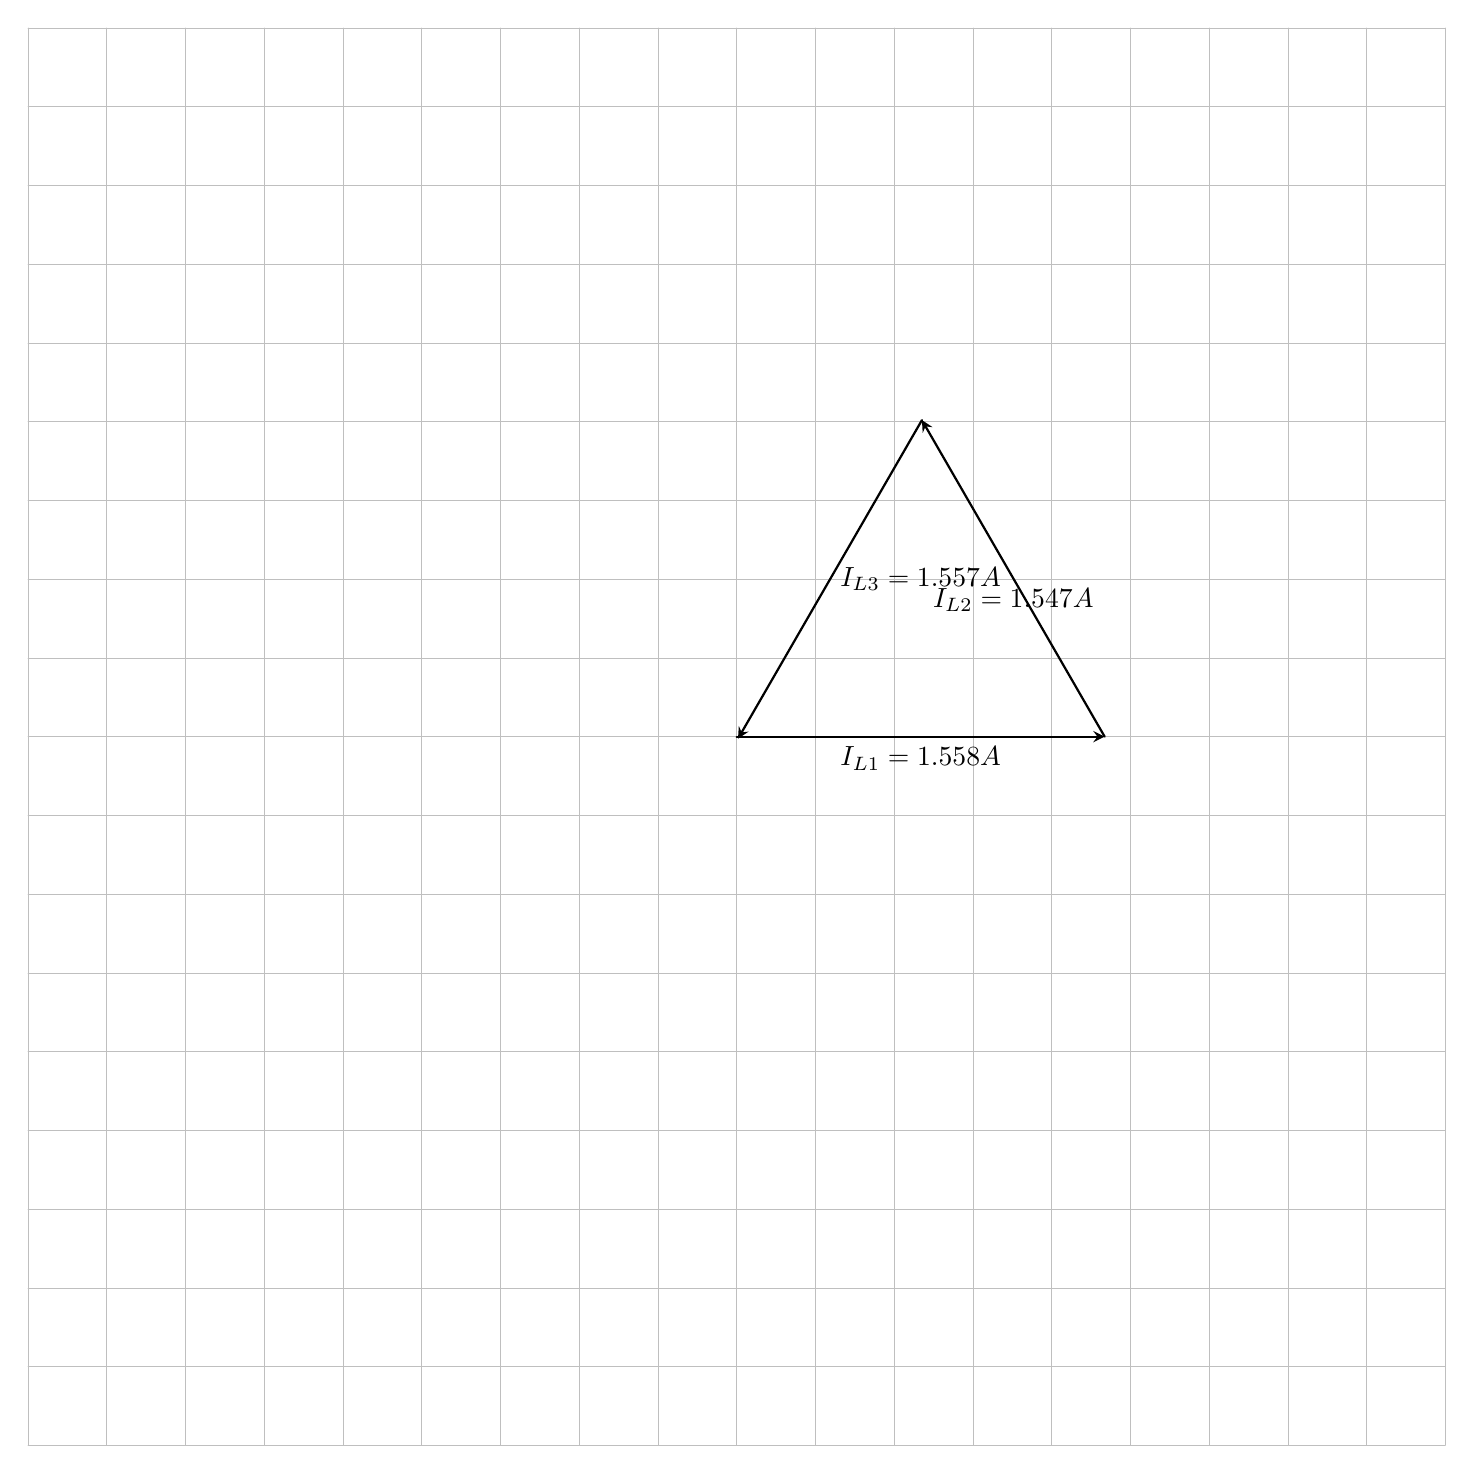
\begin{tikzpicture}[
		>=stealth,
		thick,
		line cap=round,
		line join=round
		]
		\draw[help lines,lightgray] (-9,-9) grid (9,9);
		\begin{scope}[->]
		\draw (0.0,0.0) -- (4.674,0.0) node[midway,below] {$I_{L1}=1.558A$};
		\draw (4.674,0.0) -- (2.3535000000000013,4.01922389896358) node[midway,below] {$I_{L2}=1.547A$};
		\draw (2.3535000000000013,4.01922389896358) -- (0.01800000000000246,-0.02598076211353284) node[midway,right] {$I_{L3}=1.557A$};
		\end{scope}
		\end{tikzpicture}
		\caption{Ströme des Vierleiter- Sternnetz symmetrisch}
		\label{fig:Ströme des Vierleiter- Sternnetz symmetrisch}
	\end{figure}

	\begin{figure} [H]
		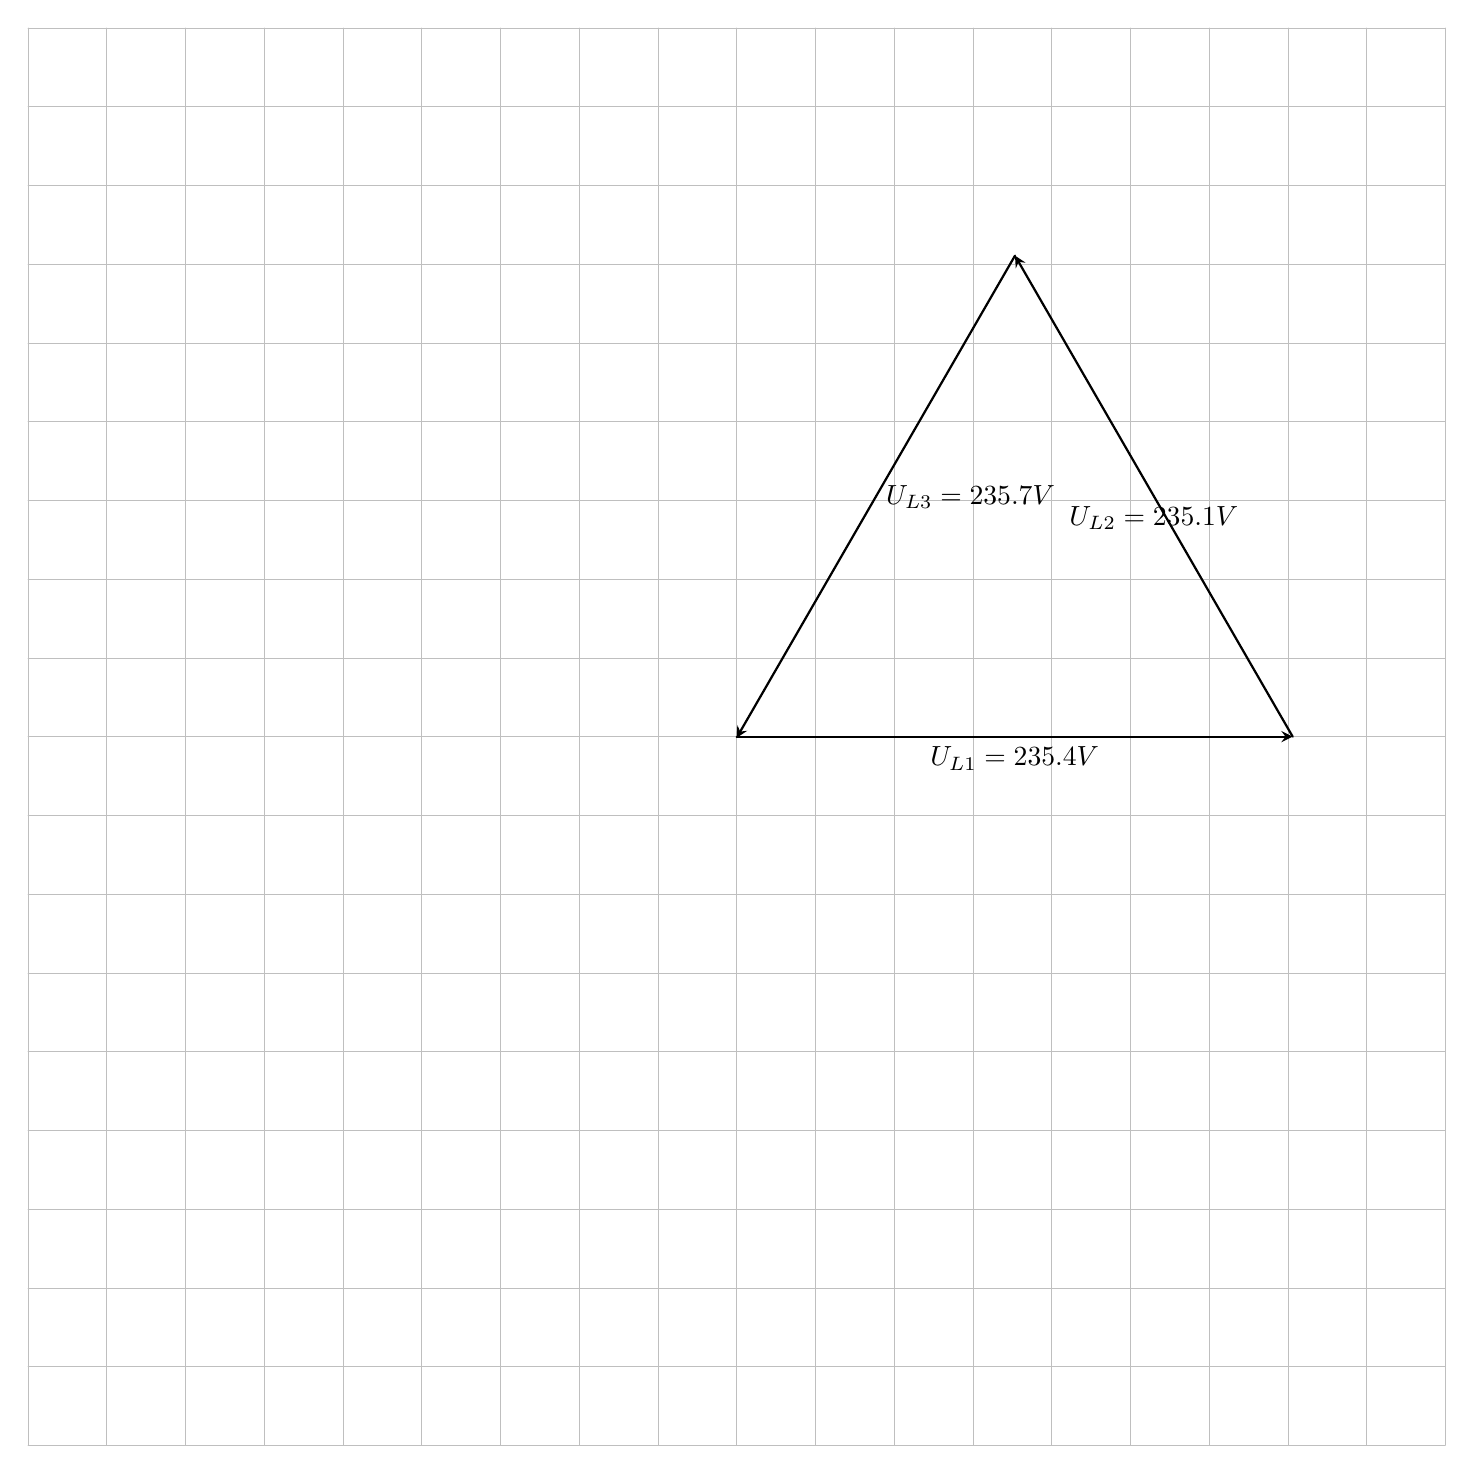
\begin{tikzpicture}[
		>=stealth,
		thick,
		line cap=round,
		line join=round
		]
		\draw[help lines,lightgray] (-9,-9) grid (9,9);
		\begin{scope}[->]
		\draw (0.0,0.0) -- (7.062,0.0) node[midway,below] {$U_{L1}=235.4V$};
		\draw (7.062,0.0) -- (3.535500000000002,6.1080771728916465) node[midway,below] {$U_{L2}=235.1V$};
		\draw (3.535500000000002,6.1080771728916465) -- (3.9968028886505635E-15,-0.015588457268119527) node[midway,right] {$U_{L3}=235.7V$};
		\end{scope}
		\end{tikzpicture}
		\caption{Spannungen des Vierleiter-Sternnetz symmetrisch}
		\label{fig:Spannungen des Vierleiter-Sternnetz symmetrisch}
	\end{figure}


	\subsubsection{Symmetrische Belastung ohne Neutralleiter}

	Durch die Entfernung des Neutralleiters entstand ein Dreileiternetz. Danach wurden ebenfalls die Strangströme $I_{L1}$, $I_{L2}$ und $I_{L3}$ sowie die umgesetzte Leistung $P_{Stern}$ gemessen.

	\begin{figure} [H]
		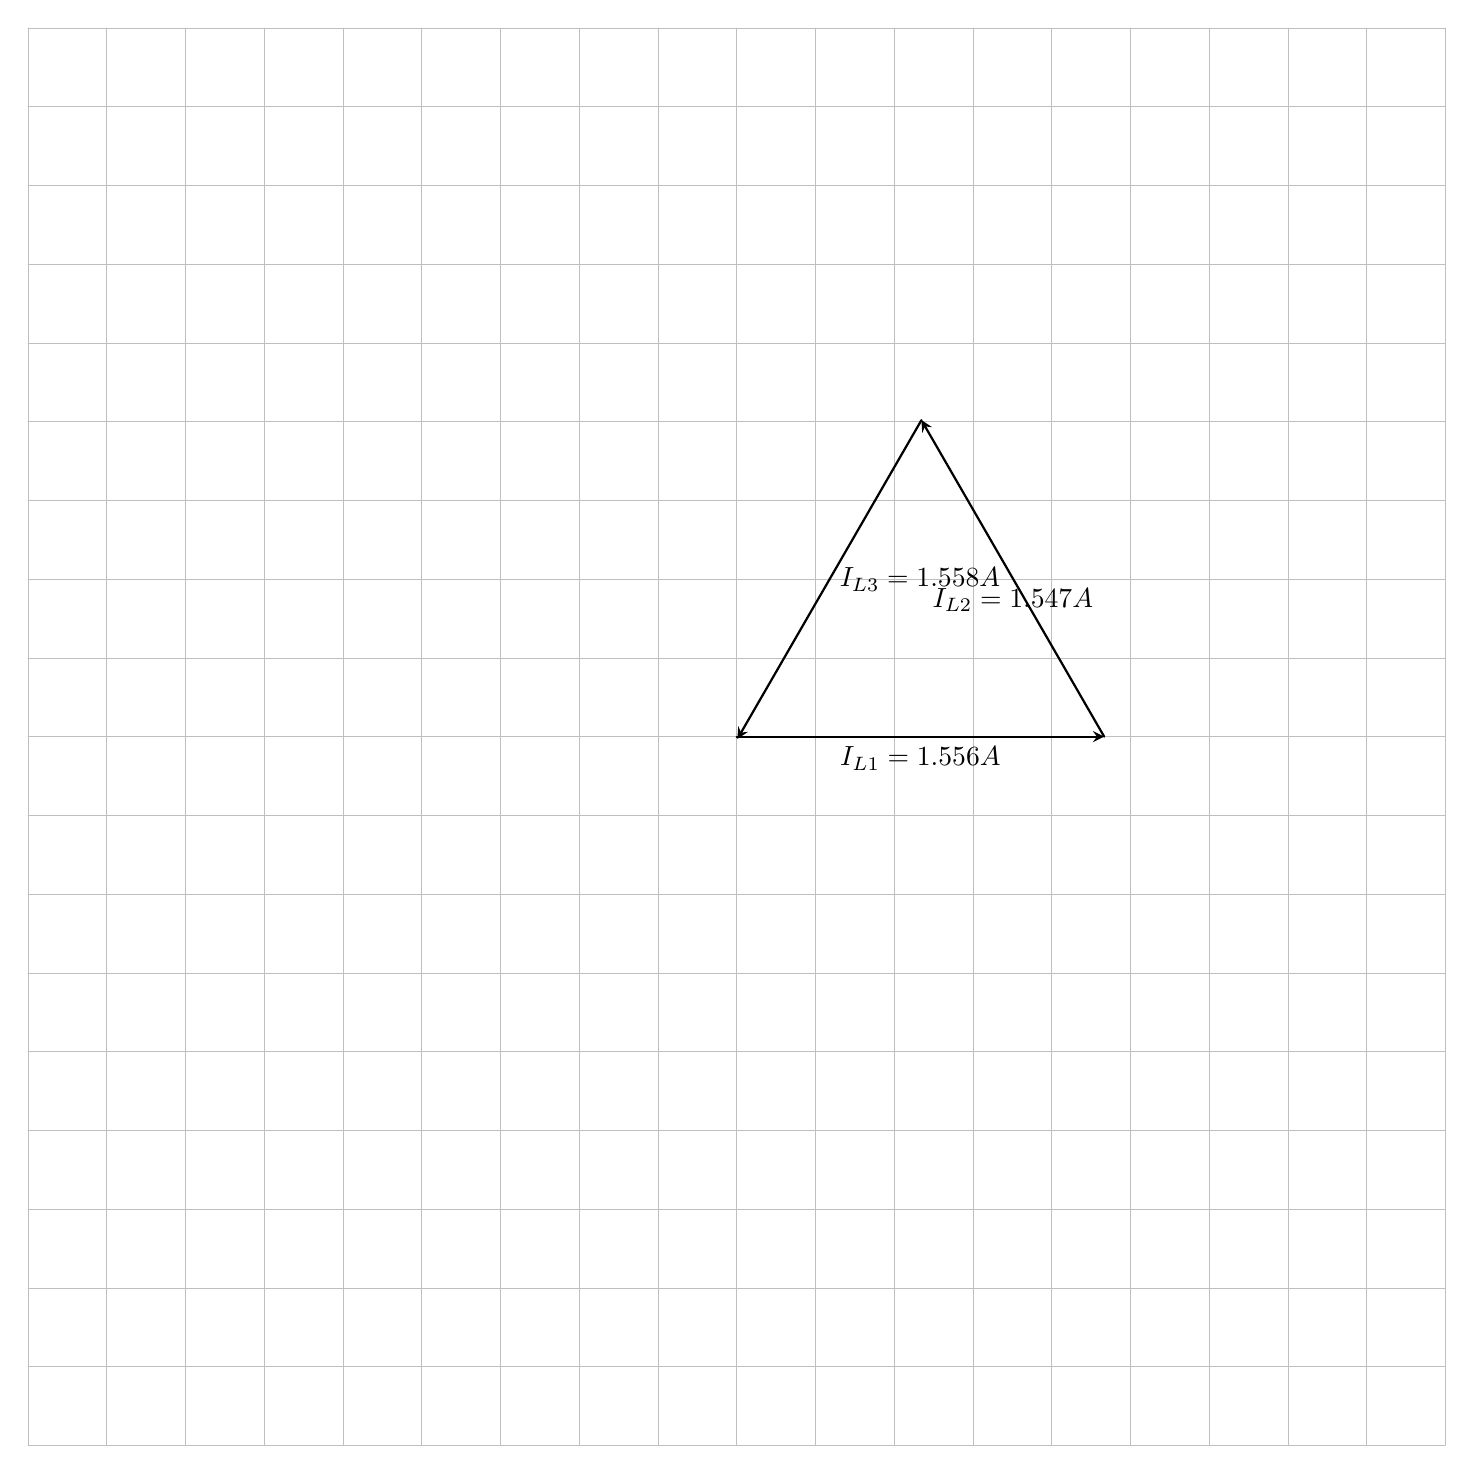
\begin{tikzpicture}[
		>=stealth,
		thick,
		line cap=round,
		line join=round
		]
		\draw[help lines,lightgray] (-9,-9) grid (9,9);
		\begin{scope}[->]
		\draw (0.0,0.0) -- (4.668,0.0) node[midway,below] {$I_{L1}=1.556A$};
		\draw (4.668,0.0) -- (2.347500000000001,4.01922389896358) node[midway,below] {$I_{L2}=1.547A$};
		\draw (2.347500000000001,4.01922389896358) -- (0.01050000000000173,-0.02857883832488639) node[midway,right] {$I_{L3}=1.558A$};
		\end{scope}
		\end{tikzpicture}
		\caption{Ströme des Dreileiter Sternnetz symmetrisch}
		\label{fig:Ströme des Dreileiter Sternnetz symmetrisch ohne Nautralleiter}
	\end{figure}


	\begin{figure} [H]
		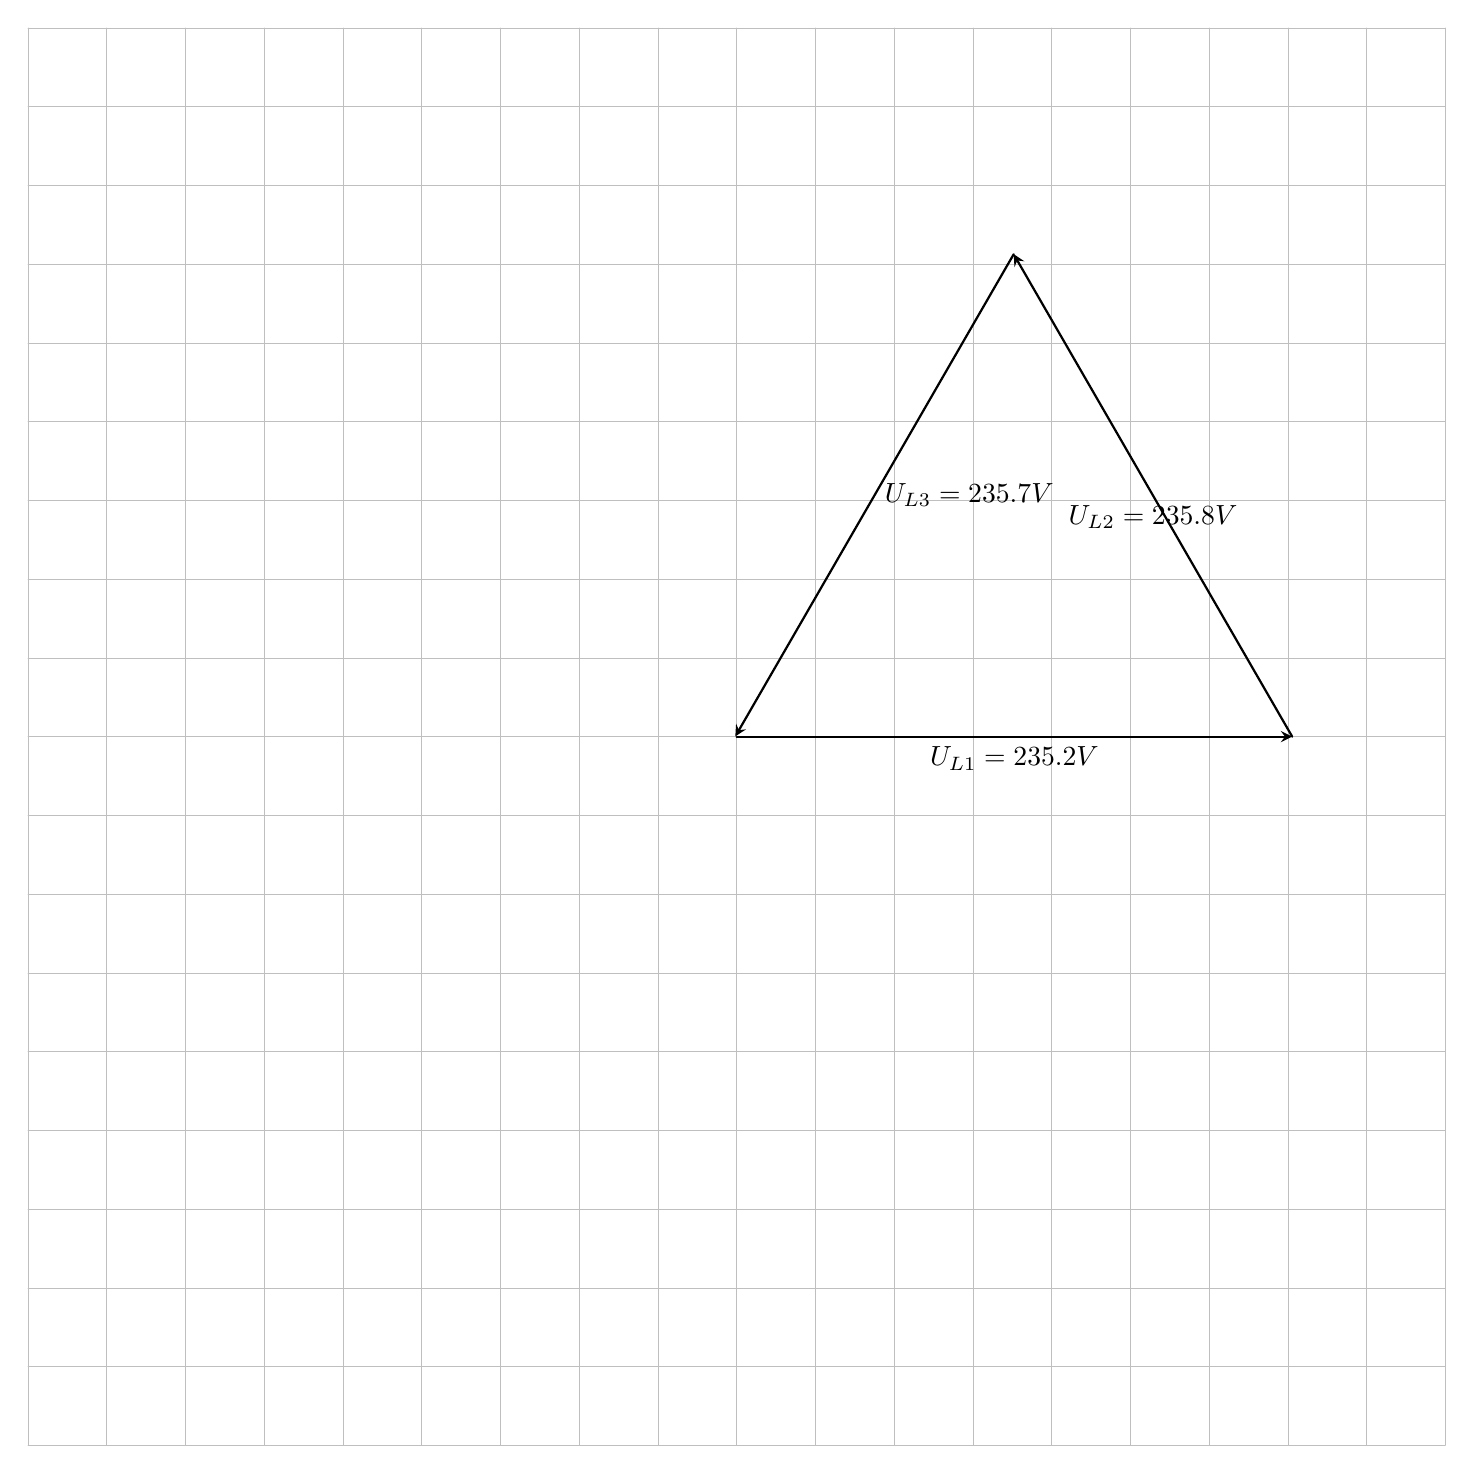
\begin{tikzpicture}[
		>=stealth,
		thick,
		line cap=round,
		line join=round
		]
		\draw[help lines,lightgray] (-9,-9) grid (9,9);
		\begin{scope}[->]
		\draw (0.0,0.0) -- (7.055999999999999,0.0) node[midway,below] {$U_{L1}=235.2V$};
		\draw (7.055999999999999,0.0) -- (3.519000000000001,6.12626370637112) node[midway,below] {$U_{L2}=235.8V$};
		\draw (3.519000000000001,6.12626370637112) -- (-0.016499999999997073,0.0025980762113535505) node[midway,right] {$U_{L3}=235.7V$};
		\end{scope}
		\end{tikzpicture}
		\caption{Spannungen des Dreileiter Sternnetz symmetrisch}
		\label{fig:Spannungen des Dreileiter Sternnetz symmetrisch ohne Nautralleiter}
	\end{figure}






	\subsubsection{Asymmetrische Belastung mit Neutralleiter}

	Die beiden Messungen wurden mit drei unterschiedlichen Widerstandswerten für $R_{1}$, $R_{2}$ und $R_{3}$ wiederholt. Danach wurden die Zeigerdiagramme für Ströme und Spannungen gezeichnet. Außerdem wurde die Sternpunktverschiebung gemessen. Auch dieses Mal wurde die umgesetzte Leistung $P_{Stern}$ gemessen und berechnet.

	\begin{figure} [H]
		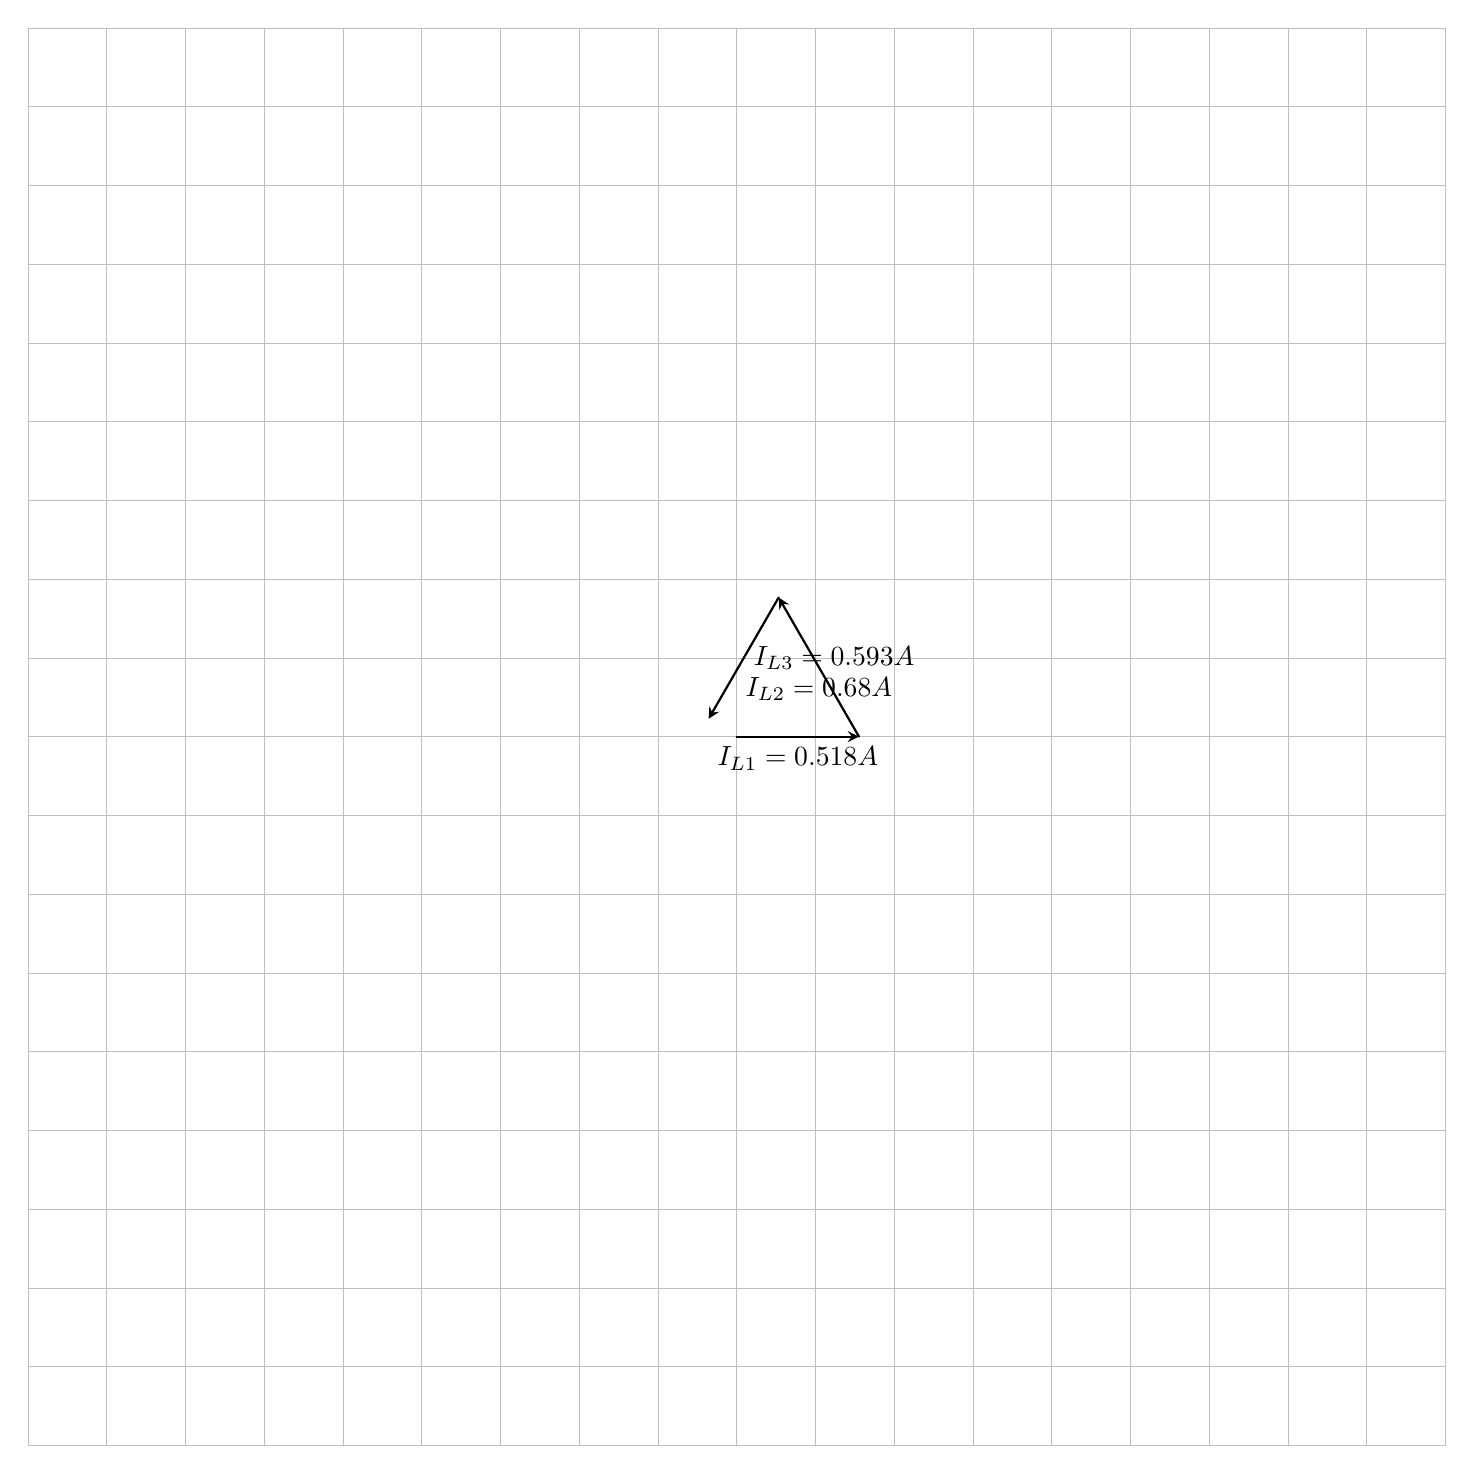
\begin{tikzpicture}[
		>=stealth,
		thick,
		line cap=round,
		line join=round
		]
		\draw[help lines,lightgray] (-9,-9) grid (9,9);
		\begin{scope}[->]
		\draw (0.0,0.0) -- (1.554,0.0) node[midway,below] {$I_{L1}=0.518A$};
		\draw (1.554,0.0) -- (0.5340000000000005,1.766691823720255) node[midway,below] {$I_{L2}=0.68A$};
		\draw (0.5340000000000005,1.766691823720255) -- (-0.35549999999999904,0.22603263038773846) node[midway,right] {$I_{L3}=0.593A$};
		\end{scope}
		\end{tikzpicture}
		\caption{Ströme des Dreileiter Sternnetz asymmetrisch mit Neutralleiter}
		\label{fig:Ströme des Dreileiter Sternnetz asymmetrisch mit Neutralleiter}
	\end{figure}

	\begin{figure} [H]
		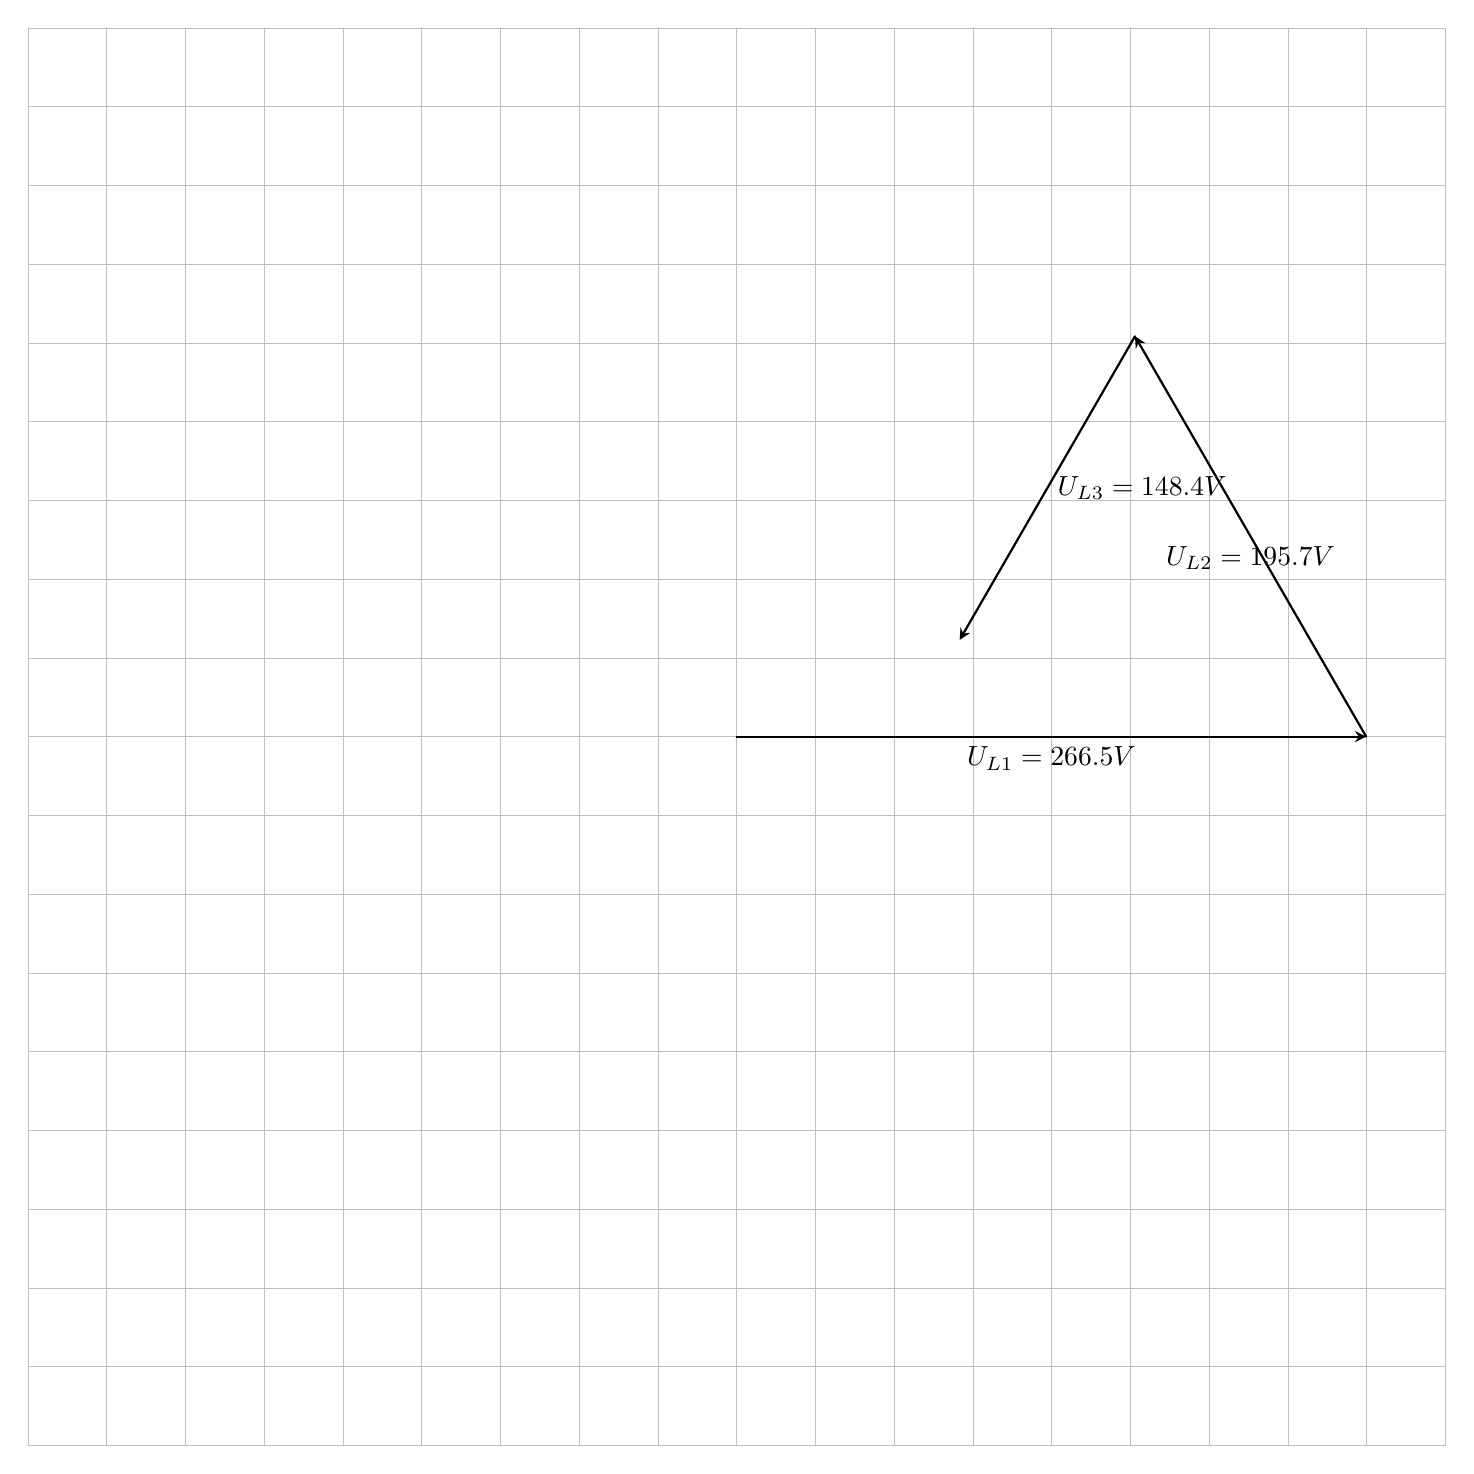
\begin{tikzpicture}[
		>=stealth,
		thick,
		line cap=round,
		line join=round
		]
		\draw[help lines,lightgray] (-9,-9) grid (9,9);
		\begin{scope}[->]
		\draw (0.0,0.0) -- (7.995,0.0) node[midway,below] {$U_{L1}=266.5V$};
		\draw (7.995,0.0) -- (5.059500000000002,5.084435145618439) node[midway,below] {$U_{L2}=195.7V$};
		\draw (5.059500000000002,5.084435145618439) -- (2.8335000000000026,1.228890047970118) node[midway,right] {$U_{L3}=148.4V$};
		\end{scope}
		\end{tikzpicture}
		\caption{Spannungen des Dreileiter Sternnetz symmetrisch}
		\label{fig:Spannungen des Dreileiter Sternnetz symmetrisch}
	\end{figure}





	\subsubsection{Asymmetrische Belastung ohne Neutralleiter}

	Die beiden Messungen wurden mit drei verschiedenen Widerstandswerten für $R_{1}$, $R_{2}$ und $R_{3}$ wiederholt. Danach wurden die Zeigerdiagramme für Ströme und Spannungen gezeichnet. Außerdem wurde die Sternpunktverschiebung gemessen. Auch dieses Mal wurde die umgesetzte Leistung $P_{Stern}$ gemessen und berechnet.

	\begin{figure} [H]
		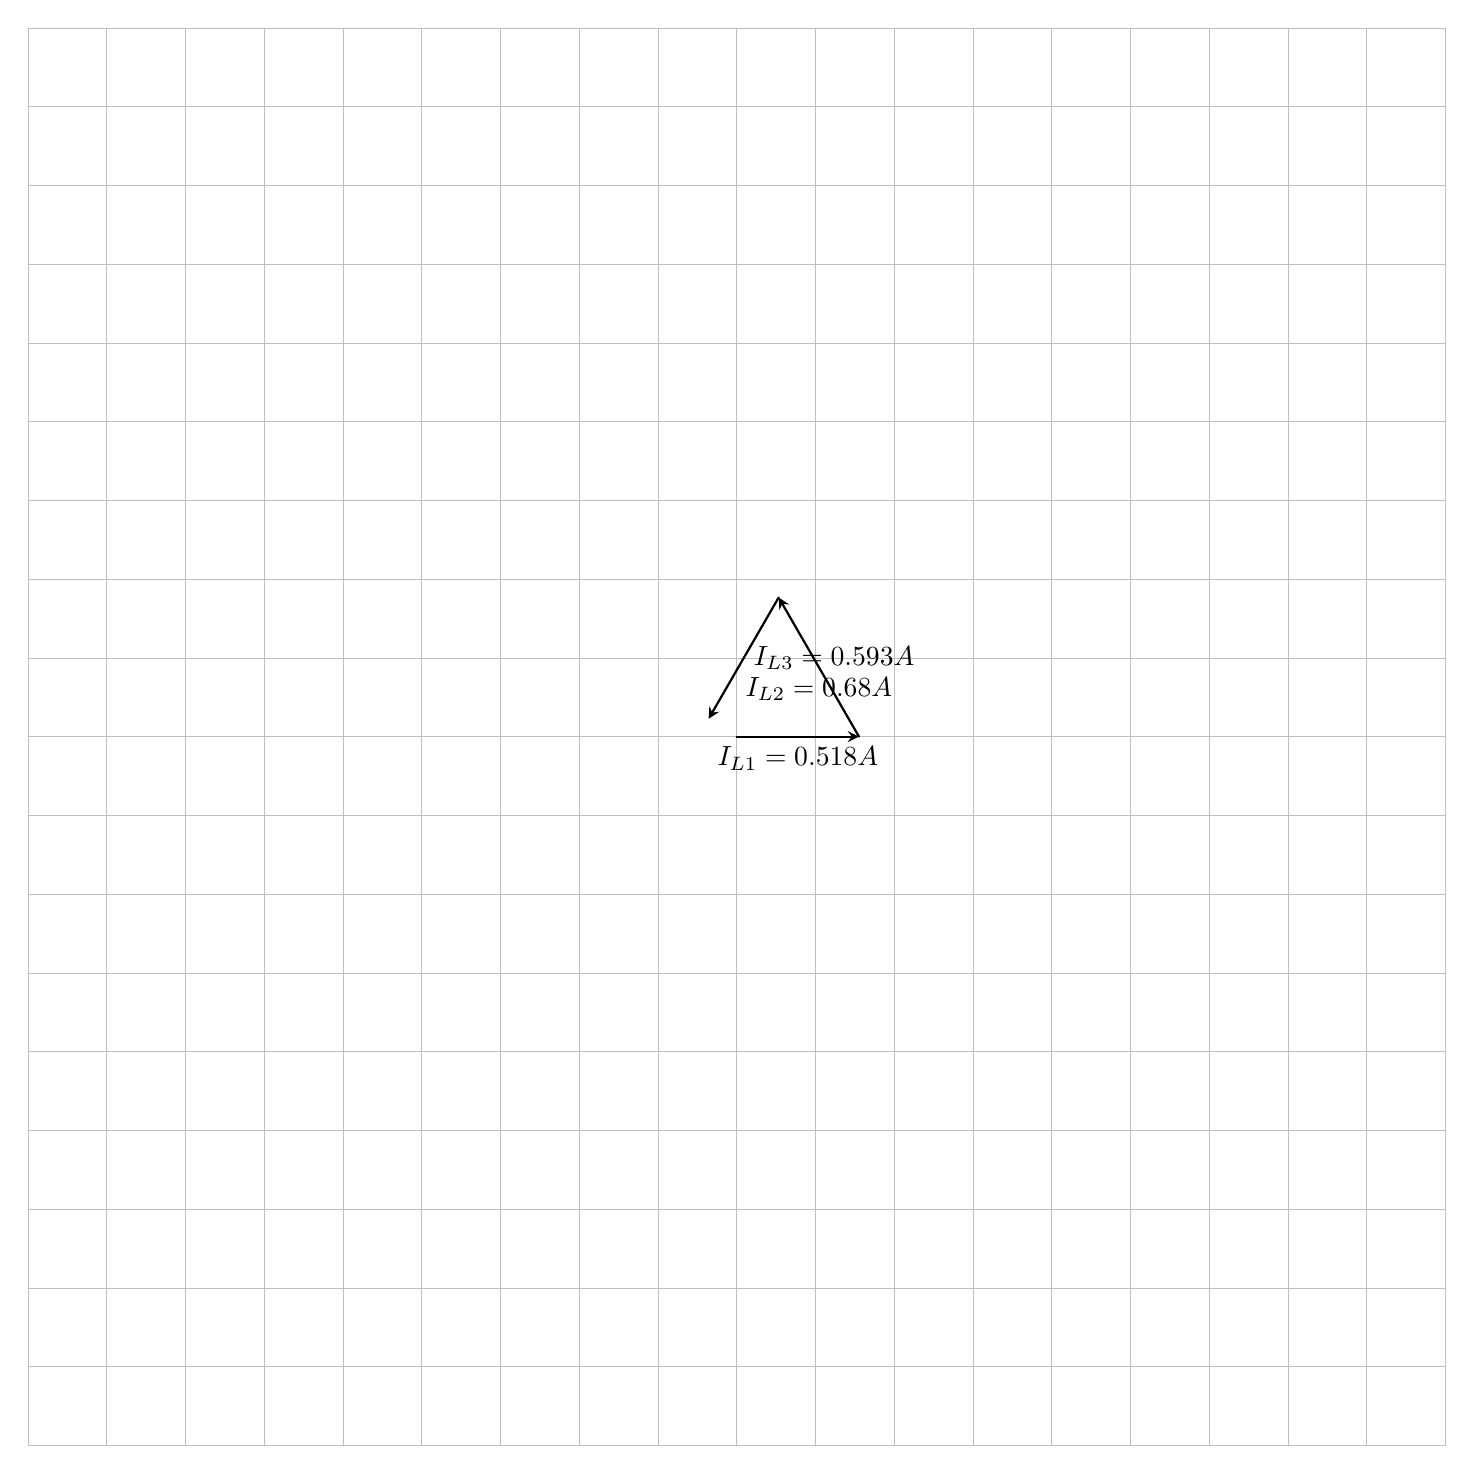
\begin{tikzpicture}[
		>=stealth,
		thick,
		line cap=round,
		line join=round
		]
		\draw[help lines,lightgray] (-9,-9) grid (9,9);
		\begin{scope}[->]
		\draw (0.0,0.0) -- (1.554,0.0) node[midway,below] {$I_{L1}=0.518A$};
		\draw (1.554,0.0) -- (0.5340000000000005,1.766691823720255) node[midway,below] {$I_{L2}=0.68A$};
		\draw (0.5340000000000005,1.766691823720255) -- (-0.35549999999999904,0.22603263038773846) node[midway,right] {$I_{L3}=0.593A$};
		\end{scope}
		\end{tikzpicture}
		\caption{Ströme des Dreileiter Sternnetz asymmetrisch}
		\label{fig:Ströme des Dreileiter Sternnetz asymmetrisch}
	\end{figure}


	\begin{figure} [H]
		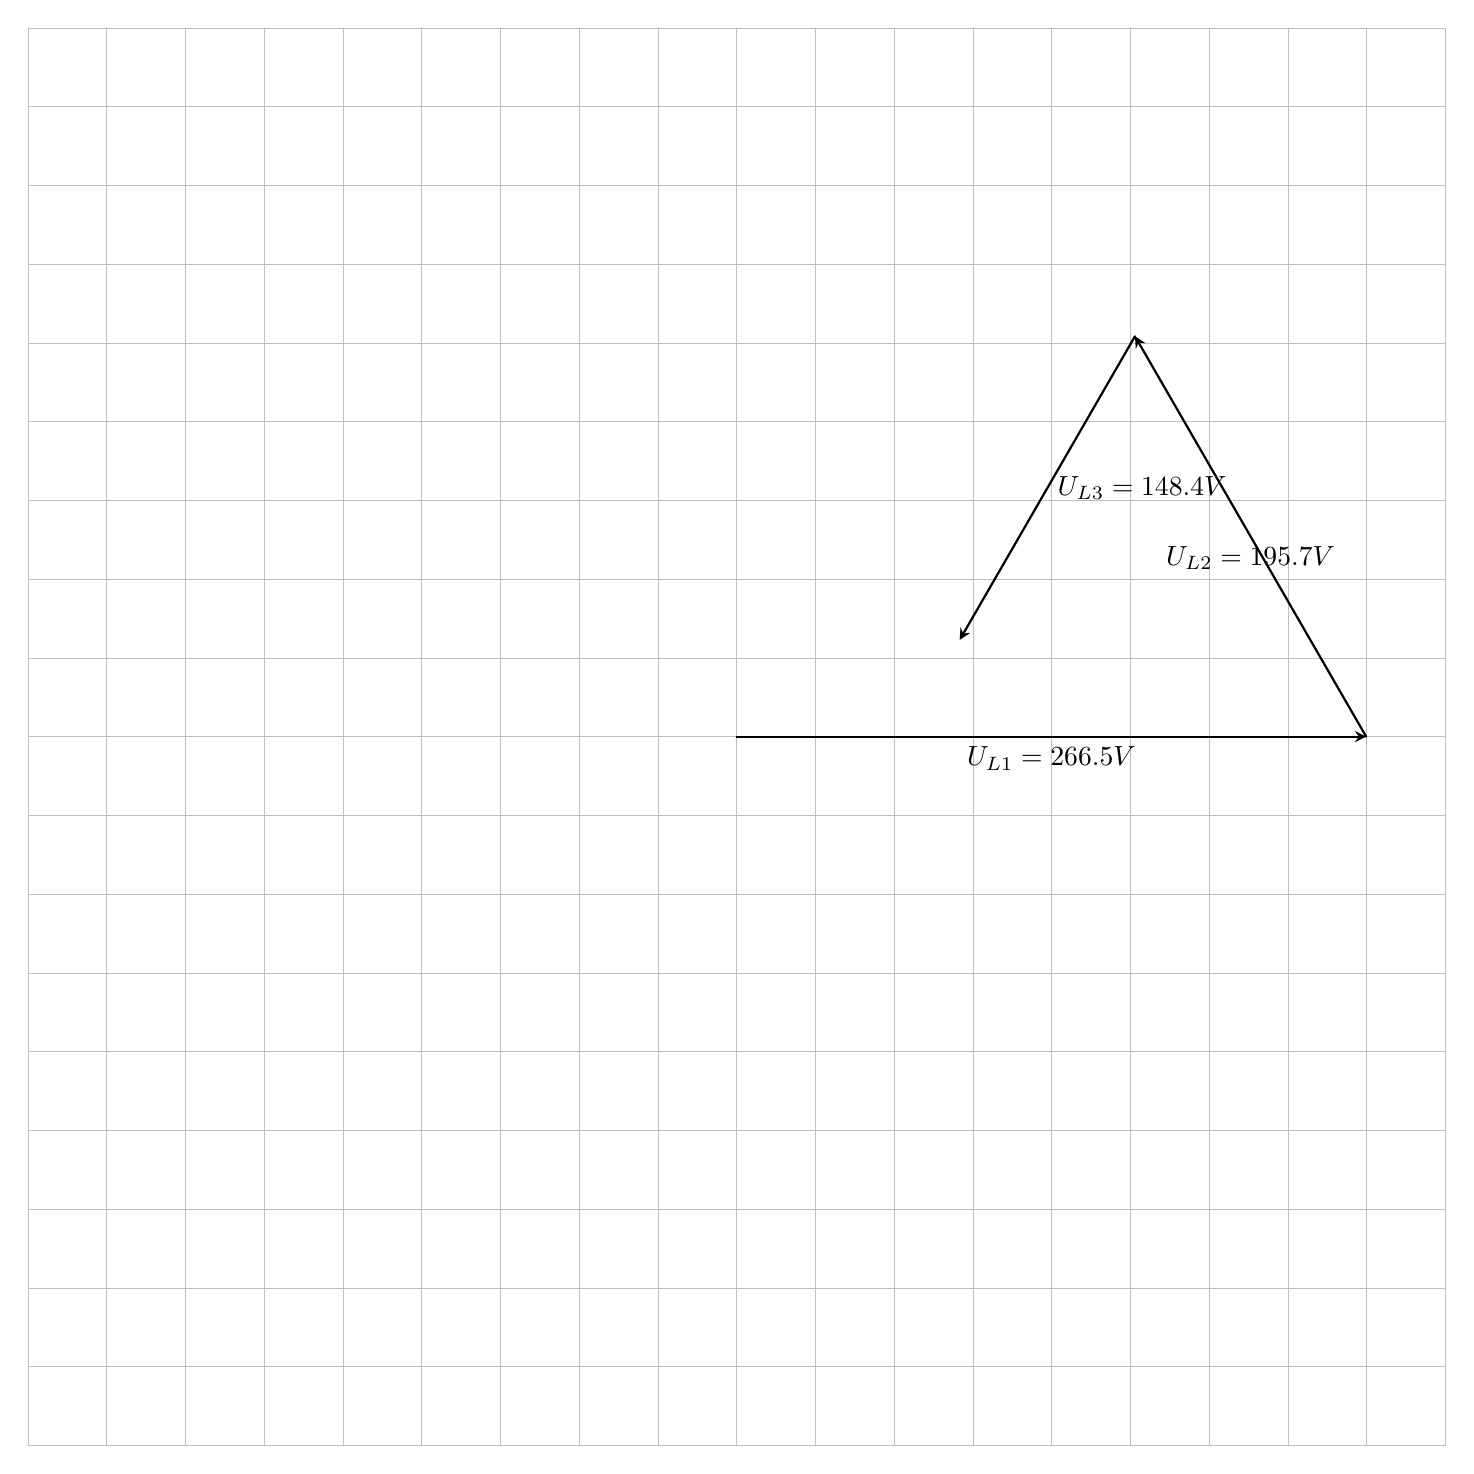
\begin{tikzpicture}[
		>=stealth,
		thick,
		line cap=round,
		line join=round
		]
		\draw[help lines,lightgray] (-9,-9) grid (9,9);
		\begin{scope}[->]
		\draw (0.0,0.0) -- (7.995,0.0) node[midway,below] {$U_{L1}=266.5V$};
		\draw (7.995,0.0) -- (5.059500000000002,5.084435145618439) node[midway,below] {$U_{L2}=195.7V$};
		\draw (5.059500000000002,5.084435145618439) -- (2.8335000000000026,1.228890047970118) node[midway,right] {$U_{L3}=148.4V$};
		\end{scope}
		\end{tikzpicture}
		\caption{Spannungen des Dreileiter Sternnetz asymmetrisch}
		\label{fig:Spannungen des Dreileiter Sternnetz asymmetrisch}
	\end{figure}


	\subsection{Dreieckschaltung}

	\subsubsection{Symmetrische Belastung}
	Es wurde ein Dreileiternetz in Dreieck mit 3 gleichgroßen Widerständen aufgebaut. Gemessen wurde die Strangströme $I_{L1}$, $I_{L2}$ und $I_{L3}$ sowie die umgesetzten Leistungen $P_{Dreieck}$ mittels Wattmeter.

	\begin{figure} [H]
		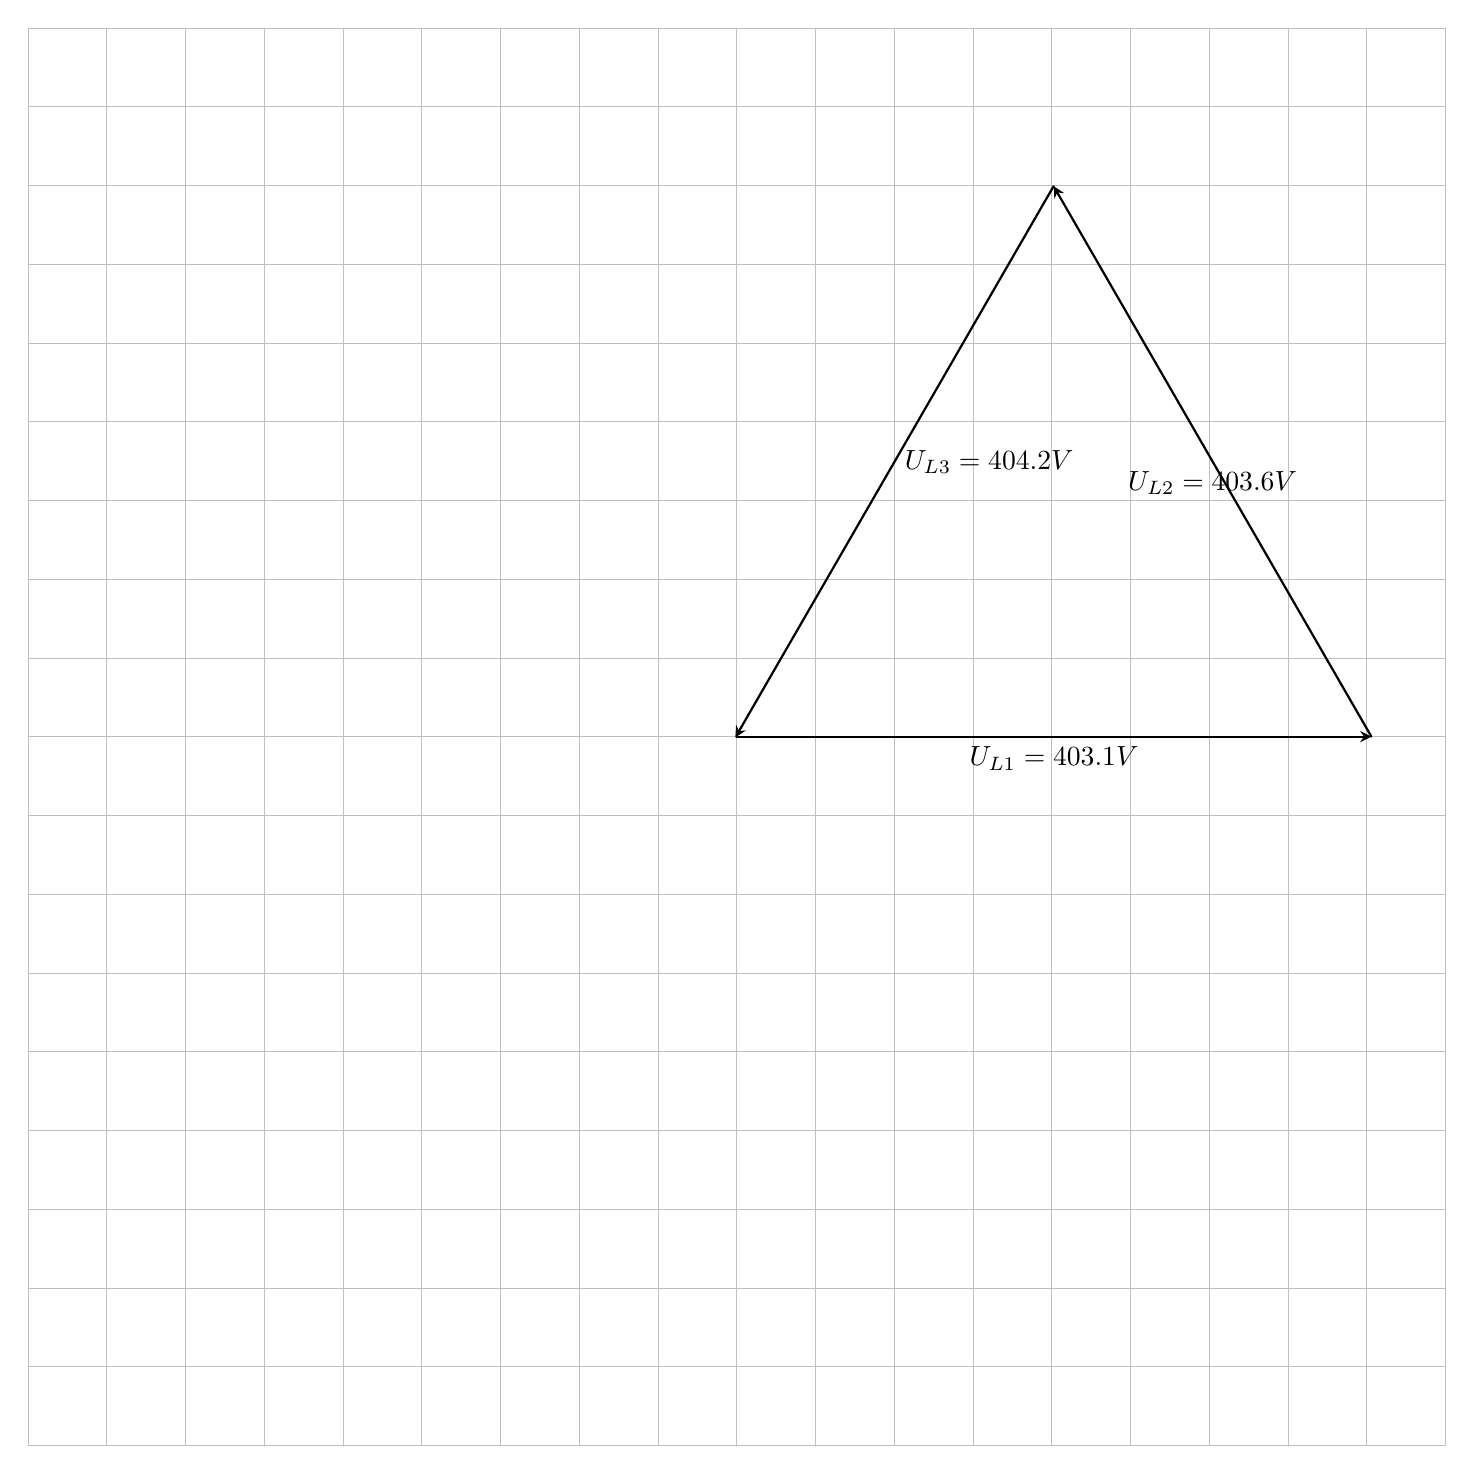
\begin{tikzpicture}[
		>=stealth,
		thick,
		line cap=round,
		line join=round
		]
		\draw[help lines,lightgray] (-9,-9) grid (9,9);
		\begin{scope}[->]
		\draw (0.0,0.0) -- (8.062000000000001,0.0) node[midway,below] {$U_{L1}=403.1V$};
		\draw (8.062000000000001,0.0) -- (4.0260000000000025,6.99055705934799) node[midway,below] {$U_{L2}=403.6V$};
		\draw (4.0260000000000025,6.99055705934799) -- (-0.015999999999995573,-0.010392304845411537) node[midway,right] {$U_{L3}=404.2V$};
		\end{scope}
		\end{tikzpicture}
		\caption{Spannungen des symmetrischen Dreileiternetzes}
		\label{fig:Spannungen des symmetrischen Dreileiternetzes}
	\end{figure}


	\begin{figure} [H]
		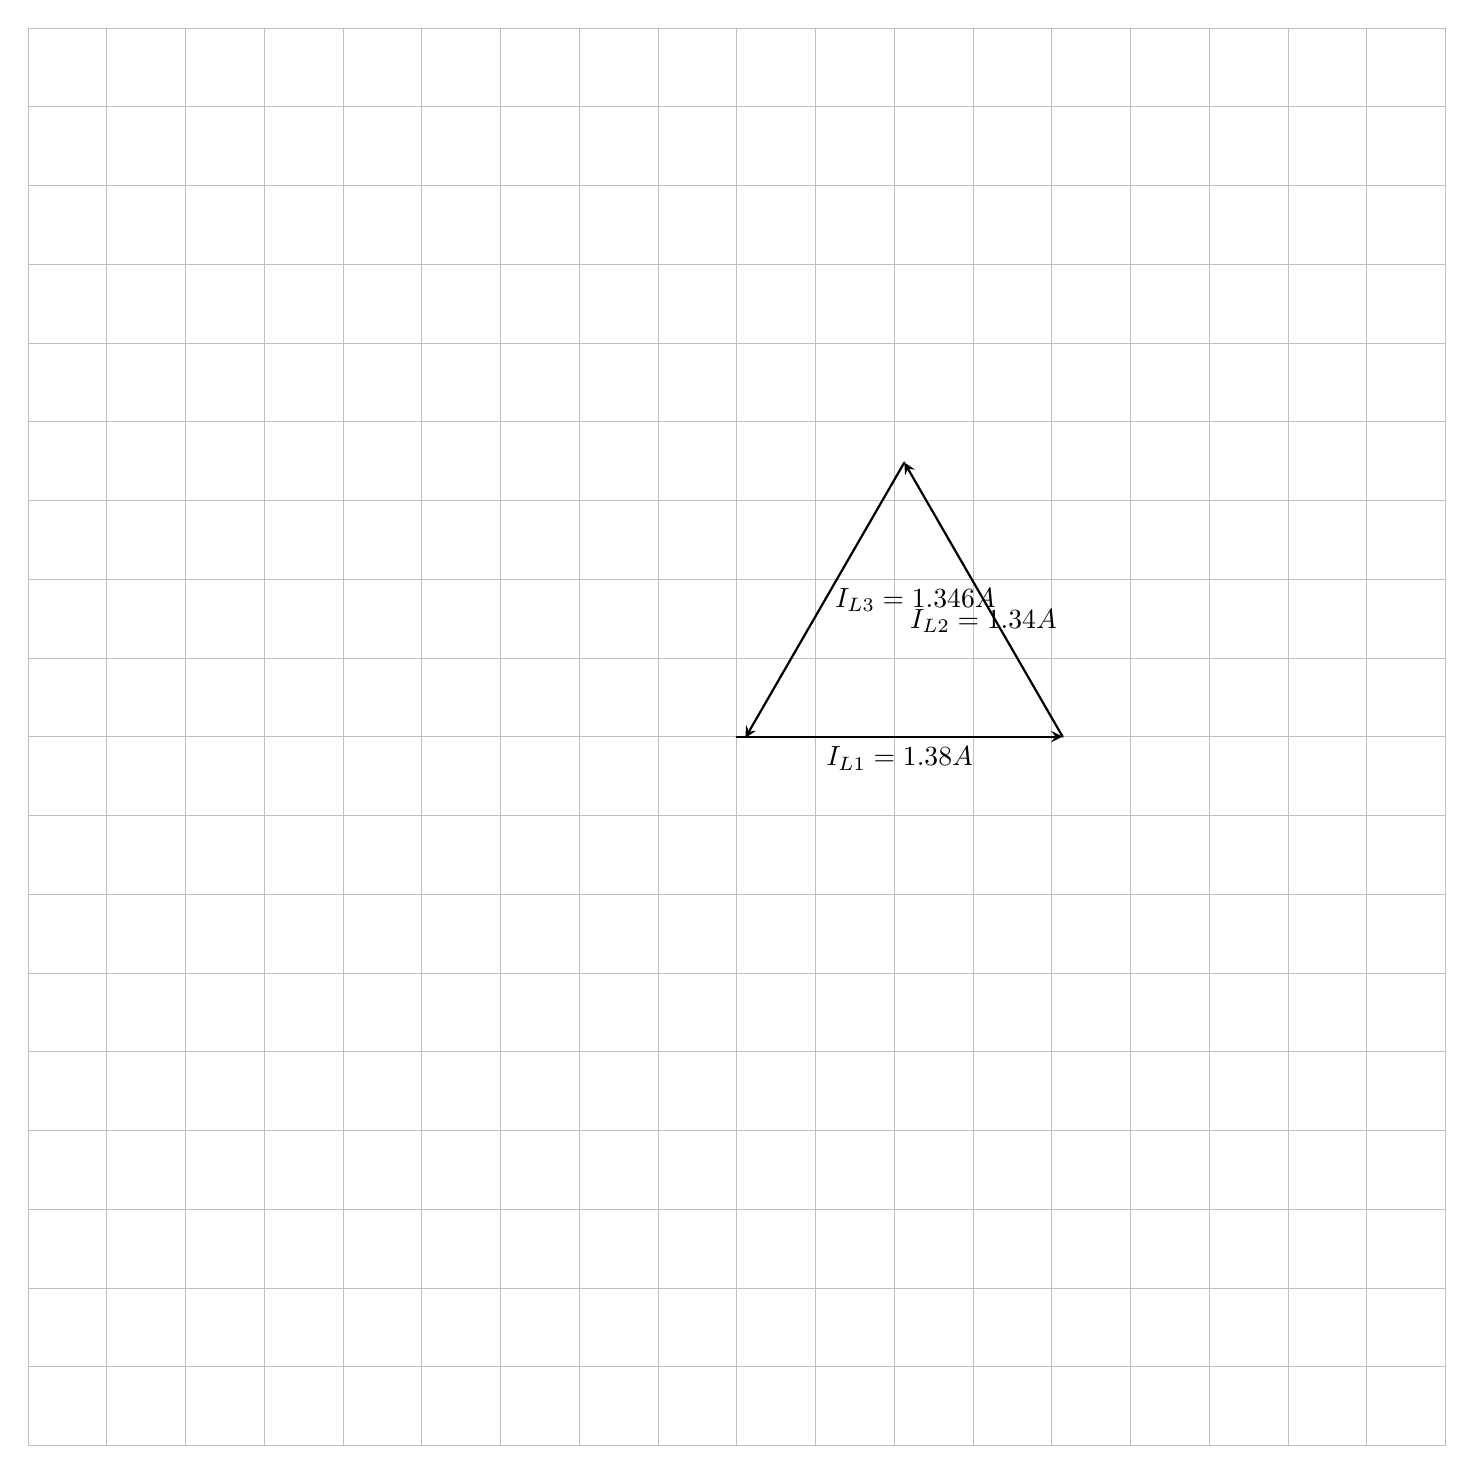
\begin{tikzpicture}[
		>=stealth,
		thick,
		line cap=round,
		line join=round
		]
		\draw[help lines,lightgray] (-9,-9) grid (9,9);
		\begin{scope}[->]
		\draw (0.0,0.0) -- (4.14,0.0) node[midway,below] {$I_{L1}=1.38A$};
		\draw (4.14,0.0) -- (2.1300000000000003,3.481422123213444) node[midway,below] {$I_{L2}=1.34A$};
		\draw (2.1300000000000003,3.481422123213444) -- (0.1110000000000011,-0.015588457268119527) node[midway,right] {$I_{L3}=1.346A$};
		\end{scope}
		\end{tikzpicture}
		\caption{Ströme des symmetrischen Dreileiternetzes}
		\label{fig:Ströme des symmetrischen Dreileiternetzes}
	\end{figure}


	\subsubsection{Asymmetrische Belastung}
	Die Messungen wurden mit drei verschiedenen Widerstandswerten für $R_{1}$, $R_{2}$ und $R_{3}$ wiederholt. Außerdem wurde die Sternpunktverschiebung gemessen. Auch dieses Mal wurde die umgesetzte Leistung $P_{Stern}$ gemessen und berechnet.

	\begin{figure} [H]
		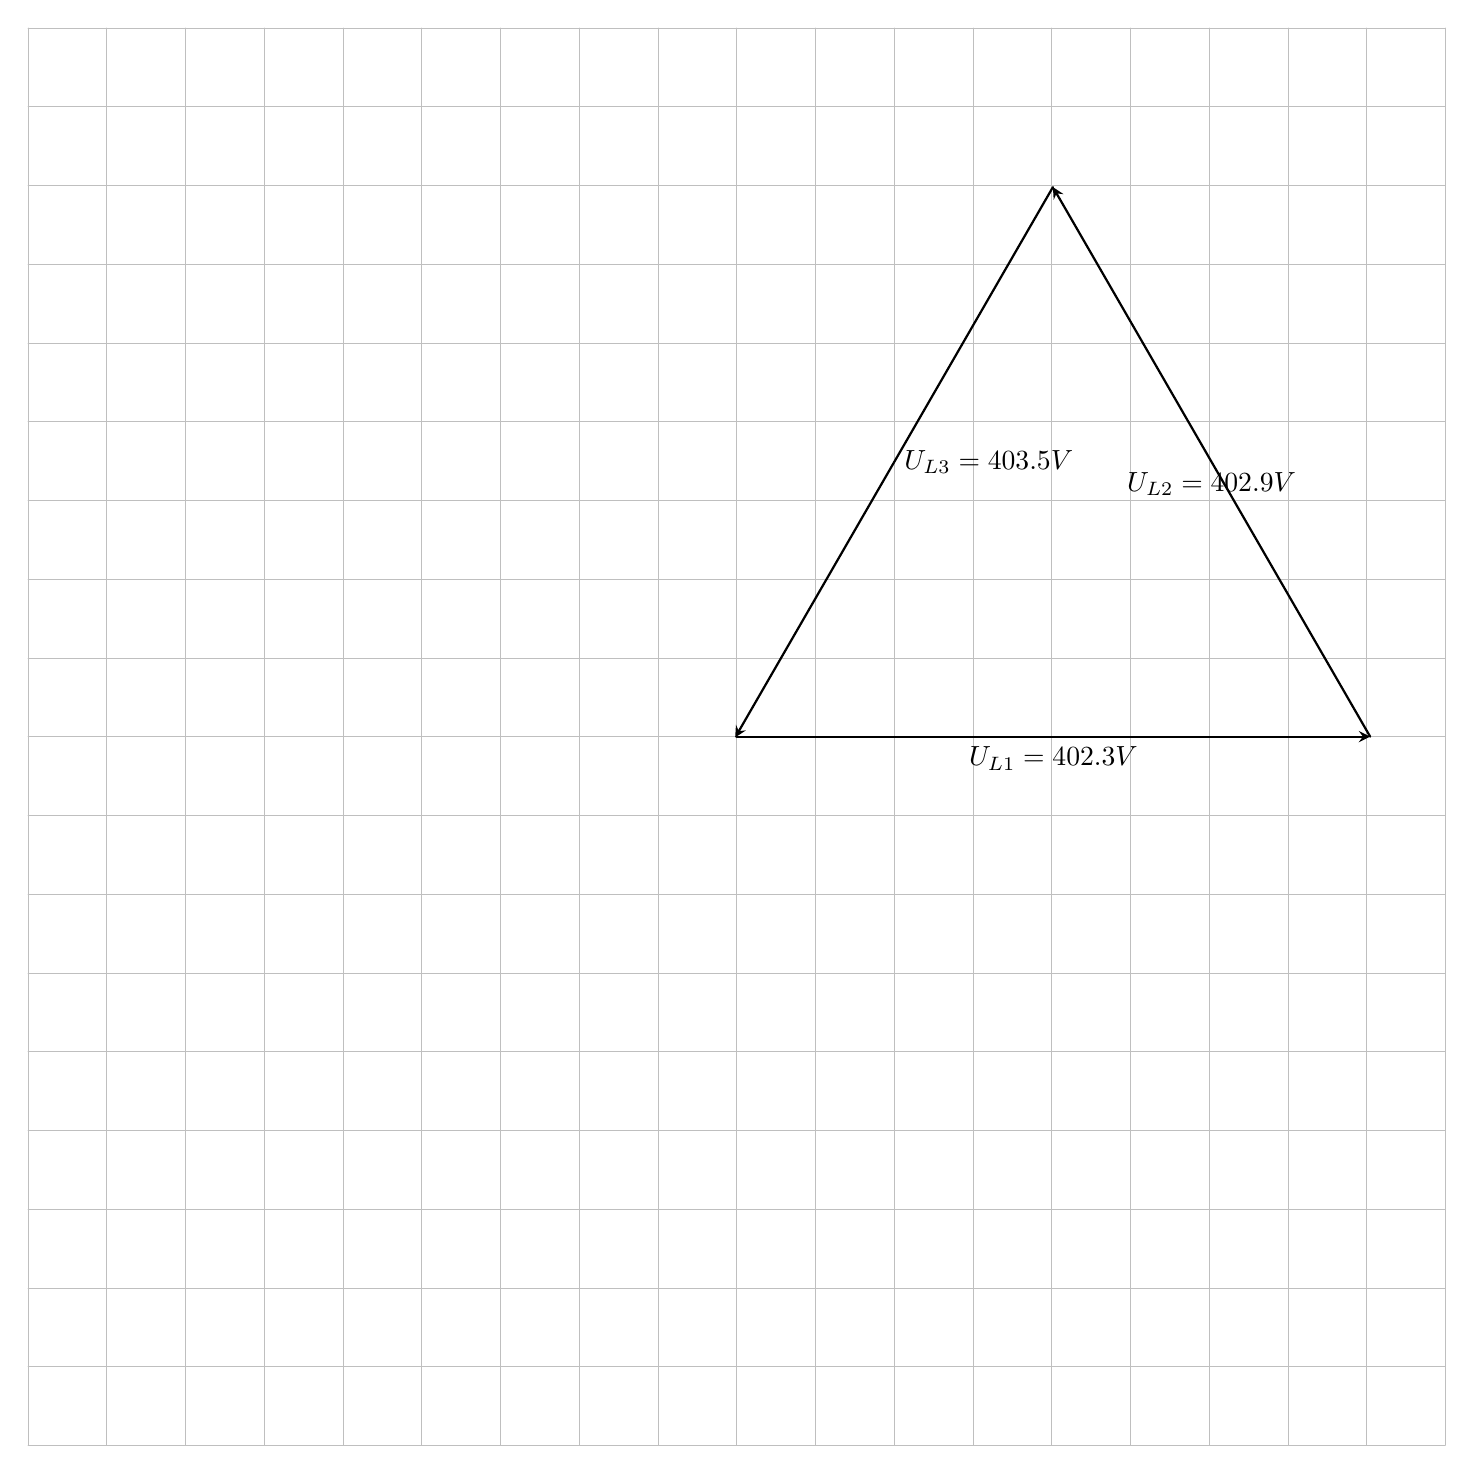
\begin{tikzpicture}[
		>=stealth,
		thick,
		line cap=round,
		line join=round
		]
		\draw[help lines,lightgray] (-9,-9) grid (9,9);
		\begin{scope}[->]
		\draw (0.0,0.0) -- (8.046000000000001,0.0) node[midway,below] {$U_{L1}=402.3V$};
		\draw (8.046000000000001,0.0) -- (4.017000000000003,6.978432703695007) node[midway,below] {$U_{L2}=402.9V$};
		\draw (4.017000000000003,6.978432703695007) -- (-0.017999999999995353,-0.010392304845413314) node[midway,right] {$U_{L3}=403.5V$};
		\end{scope}
		\end{tikzpicture}
		\caption{Spannungen des asymmetrischen Dreileiternetzes}
		\label{fig:Spannungen des asymmetrischen Dreileiternetzes}
	\end{figure}


	\begin{figure} [H]
		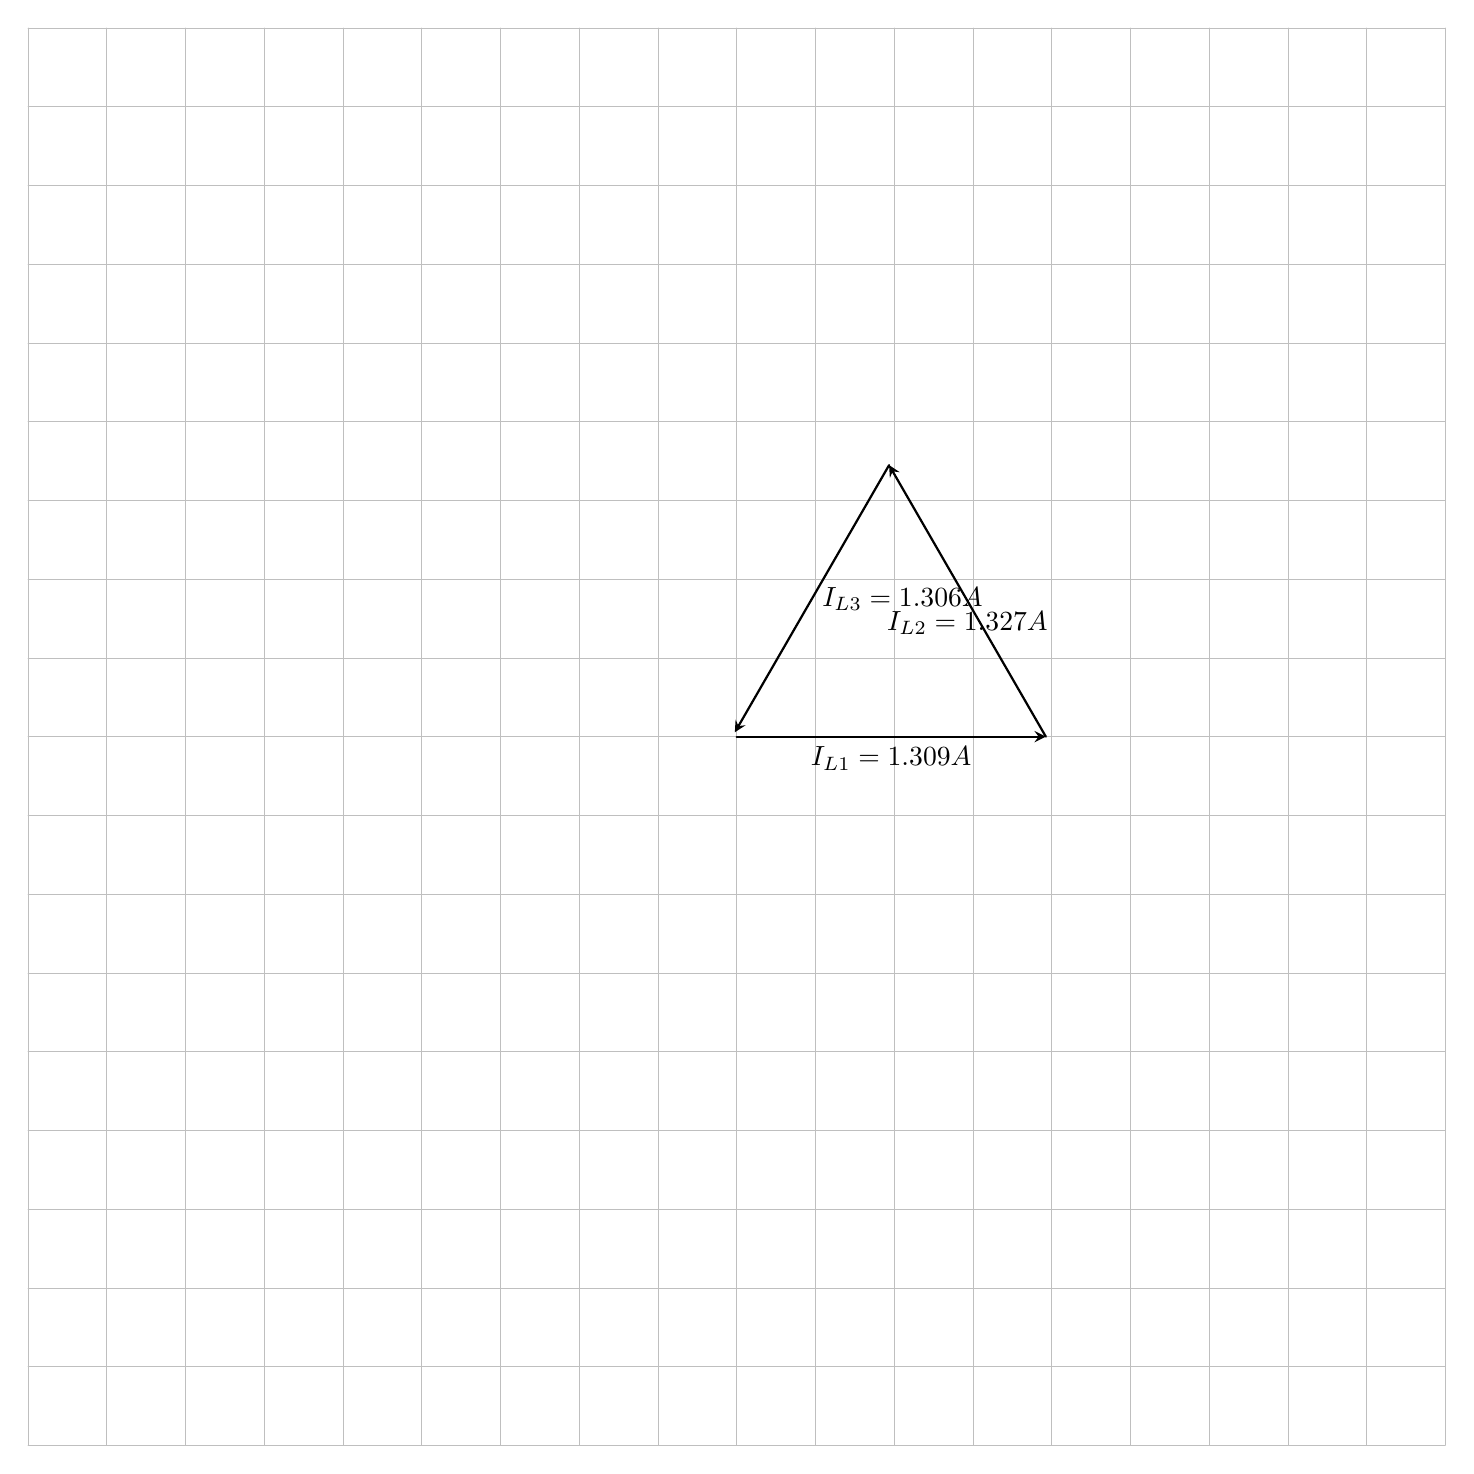
\begin{tikzpicture}[
		>=stealth,
		thick,
		line cap=round,
		line join=round
		]
		\draw[help lines,lightgray] (-9,-9) grid (9,9);
		\begin{scope}[->]
		\draw (0.0,0.0) -- (3.9269999999999996,0.0) node[midway,below] {$I_{L1}=1.309A$};
		\draw (3.9269999999999996,0.0) -- (1.9365000000000006,3.44764713246585) node[midway,below] {$I_{L2}=1.327A$};
		\draw (1.9365000000000006,3.44764713246585) -- (-0.022499999999998632,0.05455960043841923) node[midway,right] {$I_{L3}=1.306A$};
		\end{scope}
		\end{tikzpicture}
		\caption{Ströme des asymmetrischen Dreileiternetzes}
		\label{fig:Ströme des asymmetrischen Dreileiternetzes}
	\end{figure}

\end{document}


